\section{Definition and Fundamental Properties of the $\chi$ Substrate}
  \label{sec:definition-and-fundamental-properties-of-the-chi-field}

  Having outlined the ontological and conceptual principles underlying Cosmochrony, we now
  introduce the fundamental quantity at the core of the framework.
  This section is devoted to defining the pre-geometric substrate $\chi$ and clarifying its role as a
  pre-geometric substrate from which effective notions of spacetime, dynamics, and physical
  observables may emerge.

  The purpose of this section is not to assume a pre-existing spacetime structure, but to
  identify the minimal properties required of $\chi$ in order to recover, in appropriate
  regimes, effective descriptions of time, space, metric geometry, and field dynamics.
  Accordingly, $\chi$ is introduced independently of any spacetime coordinates or metric
  structure, and only later related to geometric notions once a stable spacetime interpretation
  becomes meaningful.

  Throughout this section, the use of variational principles, Lagrangian formulations, or
  metric-based expressions does not imply that spacetime or a four-dimensional manifold is
  fundamental.
  Such formalisms are employed strictly as effective, coarse-grained tools to describe the
  dynamics of $\chi$ in regimes where its configurations admit a geometric interpretation.
  They should be understood as descriptive representations of the underlying pre-geometric
  dynamics, not as primary postulates of the theory.

  We begin by providing a unified conceptual definition of the $\chi$ substrate and its physical
  interpretation.
  The subsequent subsections introduce progressively more structured effective descriptions,
  including Lagrangian and metric formulations, which become applicable only once the
  underlying $\chi$ configurations support a stable spacetime regime.

  \subsection{Definition of the $\chi$ Field}
  \label{subsec:definition-of-the-chi-field}

  We postulate the existence of a single pre-geometric relational substrate, denoted $\chi$,
  which constitutes the primitive substrate of physical reality.
  The quantity $\chi$ is not defined on a pre-existing spacetime manifold and does not
  presuppose any metric, causal, or geometric structure.
  Instead, spacetime notions arise only as effective descriptions of the relational
  and dynamical properties of $\chi$ configurations.

  Ontologically, $\chi$ is not a scalar order parameter and does not possess values.
  Scalar order parameters arise only at the effective level, as coarse-grained descriptors of projected $\chi$
  configurations once a geometric regime is established.
  Dimensional quantities associated with length or time arise only at the effective level, once $\chi$
  configurations admit a geometric interpretation.
  The monotonic ordering intrinsic to $\chi$
  configurations gives rise, upon projection, to what is operationally perceived
  as temporal flow.

  Temporal ordering emerges from the global, monotonic ordering intrinsic to $\chi$ configurations across physical
  processes, establishing an intrinsic arrow of time without reference to an external temporal coordinate.
  Spatial separation, in turn, arises from relational differences between $\chi$
  configurations, giving rise to an effective notion of distance once a stable geometric
  regime is established.
  In this sense, time corresponds to ordering, while space corresponds to relational
  structure.

  At no stage is $\chi$ interpreted as a spacetime coordinate or as a material field
  propagating on spacetime.
  Spacetime coordinates and metric structure appear only as secondary, coarse-grained
  constructs, becoming meaningful when $\chi$ configurations admit a quasi-stable
  geometric interpretation.
  The spacetime metric thus functions as an emergent, effective descriptor of resistance
  to $\chi$ relaxation\footnote{The term ``relaxation'' is used here in a geometric and
  dynamical sense, and should not be confused with thermodynamic relaxation processes
  involving dissipation or entropy increase.} and of the propagation of perturbations
  within the field.

  The analogy with thermodynamic order parameters applies only at the effective level: $\chi$ itself is not an order
  parameter, but gives rise to effective order parameters once projected.
  In the Cosmochrony framework, $\chi$ therefore provides the minimal ontological basis
  from which time, space, gravitation, and quantum phenomena jointly emerge.

  In the following sections, spacetime coordinates and metric quantities will be
  introduced strictly as effective tools, valid in regimes where $\chi$ admits a stable
  geometric interpretation.

  \begin{figure}[h]
    \centering
    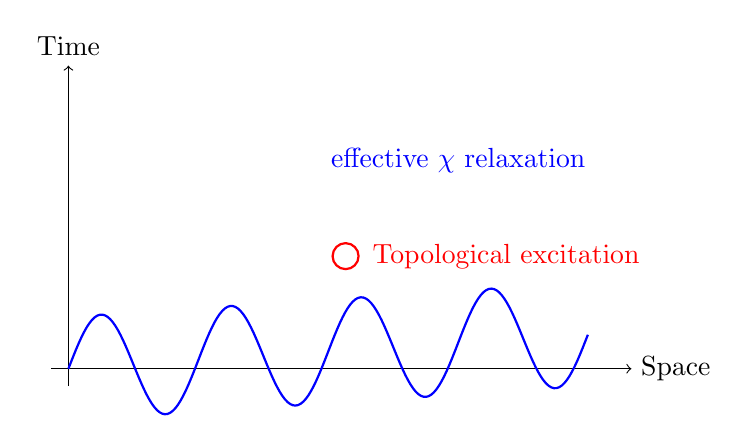
\begin{tikzpicture}[scale=1.1]

% Axes
      \draw[->] (-0.2,0) -- (6.5,0) node[right]{Space};
      \draw[->] (0,-0.2) -- (0,3.5) node[above]{Time};

% Wave
      \draw[thick, blue, domain=0:6, samples=200]
      plot (\x,{0.6*sin(2*pi*\x/1.5 r) + 0.4*\x/6});

% Particle crest
      \draw[red, thick] (3.2,1.3) circle (0.15);
      \node[red, right] at (3.4,1.3) {Topological excitation};

% Annotation
      \node[blue] at (4.5,2.4) {effective $\chi$ relaxation};

    \end{tikzpicture}
    \caption{Conceptual representation of Cosmochrony.
    An effective spacetime depiction of the projected scalar description of $\chi$,
      used for visualization purposes only.
      The monotonic relaxation of $\chi$ gives rise to an effective temporal ordering,
      while localized topological excitations correspond to particle-like configurations
      in the emergent geometric regime.}
    \label{fig:chi_concept}
  \end{figure}

  \paragraph{On the use of spacetime language.}
    Throughout this work, phrases such as ``spacetime coordinates,'' ``metric tensor,'' and ``four-dimensional
    manifold'' appear frequently, for the sake of clarity and effective description.
    These should be understood as \emph{emergent effective descriptions} valid in regimes where $\chi$
    has relaxed into a quasi-stable geometric configuration.
    They are not fundamental ingredients of the theory.

    At the deepest level, only $\chi$ and its internal relational variation structure exist.
    The appearance of familiar geometric language reflects the effectiveness of spacetime as a coarse-grained
    description of collective $\chi$
    behavior, analogous to how thermodynamic variables (temperature, pressure) emerge from molecular dynamics
    without those variables being fundamental.

    This interpretational stance is essential for distinguishing Cosmochrony from approaches that merely reformulate
    existing geometric theories in different variables.

  \subsection{The Geometric Effective Action and Lagrangians of Cosmochrony $\left(\mathcal{L}_{\mathrm{CC}}\right)$}
  \label{sec:geometric-action}

  \subsubsection*{Interpretational caution.}
    The action principle presented below employs conventional field-theoretic notation, including a metric tensor $g_{\mu \nu}$ and a four-dimensional integration measure. This should not be interpreted as assuming pre-existing spacetime structure.

    The formalism serves two purposes:
    \begin{enumerate}
      \item To provide a compact representation of $\chi$ dynamics in regimes where an effective spacetime description is valid.
      \item To establish the bridge between the fundamental relational network and the effective manifold description used in standard physics.
    \end{enumerate}

    The fundamental content of the theory is the field $\chi$ and its relaxation dynamics on a discrete graph. The metric $g_{\mu \nu}$ appearing in the action is a statistical emergent structure representing the connectivity and correlation density of the $\chi$ field, not an independent ontological input.

  \subsubsection*{Discrete Network Foundation}
    The dynamics of $\chi$ are fundamentally defined on a \textbf{discrete network}, where each node $i$ represents a local value $\chi_i$, and each link between nodes $i$ and $j$ is characterized by a \textbf{connectivity strength} $K_{ij}$. This matrix $K_{ij}$ encodes the correlation between neighboring $\chi$-values and serves as the microscopic foundation for the emergent geometry. In regimes where $\chi$ admits a quasi-stable geometric interpretation, $K_{ij}$ can be mapped to an effective metric $g_{\mu\nu}$ through the relation:
    \begin{equation}
      g_{\mu \nu} dx^\mu dx^\nu \approx \sum_{(u,v) \in \text{path}} \frac{1}{K_{uv}}
      \label{eq:metric-emergent}
    \end{equation}

  \subsubsection*{Explicit Form of the Connectivity Matrix $K_{ij}$}
    \label{subsec:Kij-definition}
    The connectivity strength $K_{ij}$ between nodes $i$ and $j$ encodes the \textbf{local correlation} between their respective $\chi$-field values. To ensure consistency with the emergent geometry and the dynamical constraints of the $\chi$ field, we adopt the following \textbf{constitutive relation}:
    \begin{equation}
      K_{ij} = K_0 \cdot f\left(\frac{|\chi_i - \chi_j|^2}{\chi_c^2}\right)
      \label{eq:Kij-def}
    \end{equation}
    where:
    \begin{itemize}
      \item $K_0$ is a \textbf{fundamental coupling scale} (with dimensions of $[\text{length}]^{-2}$), representing the maximal connectivity strength in regions where $\chi$ is uniform.
      \item $\chi_c$ is a \textbf{characteristic scale} of the $\chi$ field, naturally associated with the Planck length or the cosmological relaxation scale.
      \item $f(x)$ is a \textbf{dimensionless, monotonically decreasing function} satisfying $f(0) = 1$ and $f(x) \to 0$ as $x \to \infty$.
    \end{itemize}

    A physically motivated choice for $f(x)$ is:
    \begin{equation}
      f(x) = \frac{1}{1 + x}
    \end{equation}
    This ansatz ensures that:
    \begin{enumerate}
      \item \textbf{Symmetry}: $K_{ij} = K_{ji}$, as required for a consistent relational structure.
      \item \textbf{Locality}: $K_{ij}$ depends only on the \textbf{local difference} $|\chi_i - \chi_j|$, reflecting the pre-geometric nature of the $\chi$ field.
      \item \textbf{Boundedness}: $0 < K_{ij} \leq K_0$, preventing unphysical divergences in the emergent metric.
      \item \textbf{Gradient sensitivity}: $K_{ij}$ decreases as $|\chi_i - \chi_j|$ increases, encoding the \textbf{resistance to relaxation} induced by localized excitations (e.g., particles or curvature).
    \end{enumerate}

    This form of $K_{ij}$ provides a \textbf{microscopic foundation} for the emergent metric $g_{\mu\nu}$, as
    detailed in Section~\ref{subsec:emergent-metric}.
    The coupling scale $K_0$ and the characteristic scale $\chi_c$ are expected to be related to fundamental
    constants (e.g., the Planck length $\ell_P$ or the Hubble scale $H_0^{-1}$), but their precise values are left
    as phenomenological parameters to be constrained by observations (see Section~\ref{subsec:normalization-of-the-chi-field}).

  \subsubsection*{Emergent Geometry from $K_{ij}$}
    \label{subsec:emergent-metric}
    The connectivity matrix $K_{ij}$ defines an \textbf{operational distance} between nodes $i$ and $j$ via the minimal path sum:
    \begin{equation}
      d(i, j)^2 = \ell_0^2 \sum_{(u,v) \in \text{path}} \frac{1}{K_{uv}}
    \end{equation}
    where $\ell_0$ is a microscopic length scale (e.g., related to the Planck length).
    In the continuum limit, this discrete sum converges to the line element of an \textbf{emergent metric} $g_{\mu\nu}$:
    \begin{equation}
      ds^2 = g_{\mu\nu} dx^\mu dx^\nu \approx \ell_0^2 \left[ \delta_{\mu\nu} + \mathcal{O}\left(\frac{|\nabla \chi|^2}{\chi_c^2}\right) \right] dx^\mu dx^\nu
    \end{equation}
    Here, the corrections $\mathcal{O}(|\nabla \chi|^2 / \chi_c^2)$ encode the \textbf{curvature induced by localized excitations} (e.g., particles or black holes).
    This construction ensures that:
    \begin{itemize}
      \item \textbf{Flat spacetime} emerges when $\chi$ is uniform ($\nabla \chi = 0$), as $K_{ij} \approx K_0$ and $g_{\mu\nu} \approx \eta_{\mu\nu}$.
      \item \textbf{Curved spacetime} arises in regions where $\nabla \chi \neq 0$, as $K_{ij}$ varies spatially, inducing a non-trivial $g_{\mu\nu}$.
    \end{itemize}

    This mechanism provides a \textbf{geometric interpretation of gravity} as a modulation of the $\chi$-field's connectivity, without invoking a fundamental metric or curvature tensor.
    Further details on the continuum limit and the derivation of the effective field equations are provided in Appendix~\ref{sec:collective-coupling}.

  \subsubsection*{Effective action formulation.}
    In regimes where $\chi$ admits a quasi-stable geometric interpretation, the dynamics may be encoded in an effective action:
    \begin{equation}
      S_{\mathrm{CC}} = \int \mathcal{L}_{\mathrm{CC}} \sqrt{-g} \, d^4 x
    \end{equation}
    where the Lagrangian density decomposes as:
    \begin{equation}
      \mathcal{L}_{\mathrm{CC}} = \mathcal{L}_{\text{Gravity/Time}} + \mathcal{L}_{\chi / \text{Soliton}} + \mathcal{L}_{\text{Forces/Matter}}
    \end{equation}
    The symbol $\sqrt{-g}$ represents the invariant volume element. In regimes where no spacetime interpretation yet exists (e.g., at the nodes of the fundamental graph), this should be understood as an abstract integration measure $d\mu$ on the configuration space of $\chi$.

  \subsubsection*{Status of $g_{\mu\nu}$ in this formulation.}
    The metric $g_{\mu\nu}$ is an effective description of the coupling strengths $K_{ij}$ between $\chi$ nodes. It is defined by the requirement that the distance $ds^2$ in the continuum matches the operational distance derived from the network's connectivity:
    \begin{equation}
      g_{\mu\nu} dx^\mu dx^\nu \approx \sum_{(u,v) \in \text{path}} \frac{1}{K_{uv}}
    \end{equation}
    Consequently, $g_{\mu\nu}$ is a phenomenological summary of the underlying relational dynamics, capturing the local rate of $\chi$-relaxation and its spatial correlations.

  \subsection{Physical Interpretation}
  \label{subsec:physical-interpretation}

  In Cosmochrony, spacetime is not postulated as a fundamental background structure.
  Instead, it arises as an effective macroscopic description once configurations of
  the relational substrate $\chi$ admit a sufficiently stable and projectable regime.
  Temporal and spatial notions are therefore understood as emergent features of a
  single underlying irreversible ordering process, rather than as independent
  primitives.

  In such regimes, the infra-physical projection from $\chi$ to an effective
  description $\chi_{\mathrm{eff}}$ yields a factorisable structure, allowing an
  approximate decomposition into subsystems and the definition of operational
  observables.
  This factorisation underlies the emergence of classical locality, compatibility of
  measurements, and standard relativistic descriptions in stable domains, as
  illustrated in Fig.~\ref{fig:classical-factorisable}.

  \begin{figure}[t]
    \centering
    \begin{tikzpicture}[
      font=\small,
      node distance=10mm,
      box/.style={draw, rounded corners, align=center, inner sep=6pt},
      arrow/.style={-Latex, thick},
      note/.style={align=left, font=\footnotesize},
      dashedbox/.style={draw, dashed, rounded corners, inner sep=6pt}
    ]

    \node[box] (chi) {$\chi$\\\footnotesize infra-physical substrate};

    \node[box, below=of chi] (chieff) {$\chi_{\mathrm{eff}}$\\\footnotesize factorisable regime};

    \node[dashedbox, below=of chieff, minimum width=6.6cm] (decomp) {
      \begin{tabular}{c}
        \footnotesize $\chi_{\mathrm{eff}} \simeq \chi_{\mathrm{eff}}^{(A)} \otimes \chi_{\mathrm{eff}}^{(B)}$\\
        \footnotesize (independent subsystems)
      \end{tabular}
    };

    \node[box, below left=10mm and 12mm of decomp] (obsA) {Local observables\\in subsystem $A$};
    \node[box, below right=10mm and 12mm of decomp] (obsB) {Local observables\\in subsystem $B$};

    \draw[arrow] (chi) -- node[right=2mm, note] {infra-physical\\projection $\pi$} (chieff);
    \draw[arrow] (chieff) -- (decomp);

    \draw[arrow] (decomp) -- node[left=2mm, note] {operational\\projection $\mathcal{O}_A$} (obsA);
    \draw[arrow] (decomp) -- node[right=2mm, note] {operational\\projection $\mathcal{O}_B$} (obsB);

    \node[note, below=7mm of decomp, align=center] (compat)
    {\footnotesize Compatible operational readings: joint assignment of local observables is well-defined.};

    \end{tikzpicture}
    \caption{Classical (factorisable) regime.
    After the infra-physical projection $\pi$, the effective description
      $\chi_{\mathrm{eff}}$ admits an approximate decomposition into independent subsystems.
      Operational projections $\mathcal{O}_A$ and $\mathcal{O}_B$ then yield compatible local
      observables, recovering standard classical and relativistic descriptions.
      This figure illustrates the hierarchy between infra-physical projection and
      operational observation, and contrasts with the non-factorisable regimes discussed
      in later sections.}
    \label{fig:classical-factorisable}
  \end{figure}

  Because the projection from $\chi$ to $\chi_{\mathrm{eff}}$ is generically
  non-injective, the effective observables obtained in this way summarize relational
  structure without exhausting the underlying degrees of freedom.
  Distinct $\chi$ configurations may therefore correspond to identical effective
  descriptions, while a single underlying configuration may admit multiple correlated
  operational realizations.
  This structural asymmetry is central to the emergence of both classical and quantum
  phenomenology, and is developed in detail in subsequent sections.

  Within this interpretation, temporal ordering, relational separation, and large-scale
  behavior are not treated as independent postulates, but as complementary effective
  summaries of the same underlying relaxation dynamics, appearing at different levels
  of coarse-graining.
  Their precise operational and dynamical roles are introduced progressively in the
  following sections.

  The physical content of the theory thus resides entirely in the dynamics of the
  fundamental $\chi$ substrate, while spacetime notions function as emergent,
  context-dependent descriptive tools rather than as fundamental ingredients.

  \subsection{Monotonicity and Arrow of Time}
  \label{subsec:monotonicity-and-arrow-of-time}

  A central structural assumption of Cosmochrony is that the scalar quantity $\chi$
  evolves through a monotonic relaxation process:
  \begin{equation}
    \mathcal{D}_{\lambda} \chi \ge 0 .
  \end{equation}
  This condition is not introduced as a statistical statement, nor as a boundary
  condition imposed on an otherwise time-symmetric dynamics.
  Rather, it expresses an intrinsic property of the relaxation process governing
  $\chi$ itself.

  Within this framework, energy is not treated as a fundamental conserved substance,
  but as a measure of the remaining capacity of a given $\chi$ configuration to relax.
  As relaxation proceeds, this capacity is irreversibly expended.
  A hypothetical decrease of $\chi$ would correspond to a spontaneous restoration of
  relaxation capacity, effectively reintroducing contraction or tension into the field.
  No dynamical mechanism within Cosmochrony permits such a process.

  Irreversibility therefore follows directly from the structure of the $\chi$ dynamics.
  Because $\chi$ cannot decrease, the ordering of configurations induced by relaxation
  is intrinsically directed.
  What is conventionally described as the arrow of time is identified here with this
  directional ordering: the irreversible progression from configurations with greater
  relaxation capacity toward configurations in which that capacity has been exhausted.

  Importantly, this arrow is not derived from coarse-graining, probabilistic entropy,
  or special initial conditions.
  It emerges as a direct consequence of the monotonic relaxation of $\chi$, prior to
  any statistical or thermodynamic description.
  Temporal orientation is thus a manifestation of the fundamental dynamics, rather than
  an emergent asymmetry imposed at the macroscopic level.

  \subsection{Local Relaxation Speed}
  \label{subsec:local-relaxation-speed}

  A fundamental structural constraint of the Cosmochrony framework is that the effective
  local ordering rate associated with projected $\chi$ configurations is bounded by a
  universal constant:
  \begin{equation}
    \left| \mathcal{D}_{\mathrm{loc}} \chi_{\mathrm{eff}} \right| \le c ,
  \end{equation}
  where $\mathcal{D}_{\mathrm{loc}} \chi_{\mathrm{eff}}$ denotes an effective local
  relaxation functional characterizing the maximal admissible ordering of projected
  $\chi$ configurations within the emergent geometric description.
  The parameter $c$ coincides numerically with the observed speed of light.

  This bound does not represent the propagation speed of particles, fields, or signals,
  nor does it presuppose a pre-existing spacetime structure.
  Rather, it constrains the maximal rate at which effective causal relations and geometric
  structure can locally emerge within projected descriptions compatible with the
  underlying ordering structure of $\chi$.

  Superluminal recession velocities at cosmological scales arise naturally through
  cumulative and global effects of projected $\chi$ ordering, and do not violate local
  causality.
  Local causal relations remain bounded by the constraint $c$, which applies exclusively
  to effective descriptions and not to the fundamental $\chi$ substrate itself.

  \subsection{Relation to Conventional Fields}
  \label{subsec:relation-to-conventional-fields}

  Although effective descriptions derived from projected $\chi$ configurations may
  exhibit formal similarities with scalar fields employed in cosmology (such as
  inflaton-like fields), the ontological role of $\chi$ is fundamentally different.
  The $\chi$ substrate is not a physical field propagating on spacetime, but a
  pre-geometric relational structure from which spacetime notions themselves emerge.

  Accordingly, $\chi$ does not carry energy in the conventional field-theoretic sense,
  nor is it subject to quantization at the fundamental level.
  Quantization arises only at the effective level, where certain stable and localized
  configurations of the $\chi$ substrate admit a particle-like interpretation and can
  be consistently described using standard quantum field-theoretic tools within an
  emergent spacetime regime.

  Within this framework, matter, radiation, and interactions do not correspond to
  independent fields coupled to $\chi$.
  They arise instead as effective manifestations of constraints, topological features,
  or long-lived relational patterns of projected $\chi$ configurations.
  Conventional fields of the Standard Model are thus recovered as effective
  descriptions of these emergent degrees of freedom in regimes where a spacetime
  interpretation appl

  \subsection{Initial Conditions and Global Structure}
  \label{subsec:initial-conditions-and-global-structure}

  The Cosmochrony framework does not postulate initial conditions in the conventional
  temporal sense.
  Instead, it assumes that the relational substrate $\chi$ admits a minimal admissible
  ordering state, denoted $\chi_0$, corresponding to configurations of maximal effective
  relaxation density.
  This reference state characterizes the earliest physically meaningful configurations
  within projected descriptions, without presupposing a fundamental temporal origin or
  a distinguished initial instant.

  In effective geometric regimes, the characteristic scale associated with projected
  descriptions near $\chi_0$ coincides numerically with the Planck scale.
  This correspondence reflects the breakdown of coarse-grained spacetime descriptions
  below this regime, rather than the presence of a fundamental cutoff, discreteness, or
  microscopic spacetime structure.

  From this perspective, cosmic history is interpreted as the progressive ordering of
  projected $\chi$ configurations away from this minimal admissible state.
  No spacetime singularity is required in the fundamental description.
  Apparent singular behavior arises only when classical notions of time and distance are
  extrapolated beyond the regime in which projected $\chi$ configurations admit a
  stable geometric interpretation.

  The global structure of admissible projected descriptions is thus constrained by the
  ordering properties of the underlying $\chi$ substrate, rather than by arbitrarily
  specified initial data.
  In the following section, we derive a minimal effective dynamical equation governing
  the ordering of projected $\chi$ configurations and explore its immediate physical
  consequences.

